\documentclass[]{scrreprt}
\usepackage{amsmath,amsfonts,graphicx}
\usepackage{multirow}
\usepackage{pslatex}
\usepackage{tabularx}
\usepackage{comment}
\usepackage{xspace}
\usepackage{array}

\usepackage{hyperref}

\usepackage{caption}
\DeclareCaptionFont{white}{\color{white}}
\DeclareCaptionFormat{listing}{\colorbox{gray}{\parbox{\textwidth}{#1#2#3}}}

\graphicspath{
{figures/}
}

\newcommand{\uo}{\mbox{UO\textsubscript{2}}\xspace}

\setcounter{secnumdepth}{3}


\begin{document}


\title{Richards Tests}
\author{Andy Wilkins \\
CSIRO}
\maketitle

\tableofcontents

%%%
\chapter{Introduction}
%%%

The Richards' equation describes slow fluid flow through a porous
medium.  This document describes the test suite associated with the
Richards MOOSE code, both brief unit-style tests, and more complicated
benchmark verifications.  There are two other accompanying documents: (1)
The theoretical and numerical foundations of the code; (2) Examples of
input syntax that users can utilise when building models.


\chapter{UserObject tests}

The Richards' UserObjects define the nonlinear functions that form the
core of all models.  The tests of these UserObjects involve checking
whether the functions and their derivatives are correctly coded.  This
is done by comparing the values of the UserObjects with
ParsedFunctions that are coded into a MOOSE input file, and the values
of the UserObject derivatives with finite-differences of the same
ParsedFunction.  These are simple tests and are part of the automatic
test suite.  The following tests are performed.

\begin{itemize}

\item That the `power' form of the relative permeability:
\begin{equation}
\kappa_{\mathrm{rel}}(S) = (n+1)S^{n} - nS^{n+1} \ ,
\end{equation}
is correctly coded, and also that its first and second derivatives
with repsect to $S$ are correctly coded.

\item That the `van Genuchten' form of the relative permeability:
\begin{equation}
\kappa_{\mathrm{rel}}(S) = \sqrt{S}\left(1 - \left(1 -
S^{1/m}\right)^{m}\right)^{2} \ ,
\end{equation}
is correctly coded, and also that its first and second derivatives
with respect to $S$ are correctly coded.

\item That the 'modified van Genuchten' form of the relative permeability:
\begin{equation}
\kappa_{\mathrm{rel}}(S) = \left\{
\begin{array}{ll}
\sqrt{S}\left(1 - \left(1 -
S^{1/m}\right)^{m}\right)^{2} \ & \mbox{ for } S<S_{\mathrm{cut}} \\
\mbox{cubic} \ & \mbox{ for } S \geq S_{\mathrm{cut}}
\end{array}
\right.
\end{equation}
is correctly coded, and also that its first and second derivatives
with respect to $S$ are correctly coded.

\item That the `constant bulk modulus' form of the density
\begin{equation}
\rho(P) = \rho_{0}e^{P/B} \ ,
\end{equation}
is correctly coded, and also that its first and second derivatives
with respect to $P$ are correctly coded.

\item That the `ideal gas' form of the density
\begin{equation}
\rho(P) = s(P-P_{\mathrm{0}}) \ ,
\end{equation}
is correctly coded, and also that its first and second derivatives
with respect to $P$ are correctly coded.

\item That the `van Genuchten' effective saturation
\begin{equation}
S_{\mathrm{eff}} = \left(1 + (\alpha
P_{\mathrm{c}})^{\frac{1}{1-m}}\right)^{-m} \ ,
\end{equation}
is correctly coded, and also that its first and second derivatives
with respect to $P_{\mathrm{c}}$ are correctly coded.

\end{itemize}



\chapter{Jacobian tests}

The UserObjects and their derivatives need to be combined to form a
residual and a Jacobian during the solution process.  Correctly coding
the Jacobian leads to rapid convergence to the correct solution, so
tests of the Jacobian are important.  These are simple tests and are
part of the automatic test suite.

In MOOSE parlance, the Jacobian consists of `Diagonal' and
`OffDiagonal' terms.  The former consist of the derivative of a
variable's residual with respect to the same variable (at the same
quadrature point or a different one); while the latter
consist of the derivatives with respect to another variable (at the
same quadrature point or a different one).

The `Diagonal' terms are tested using a single-phase single-element
model with random initial conditions.  Sixteen different tests are
performed which are all possible combinations of:
\begin{itemize}
\item Fully-saturated or unsaturated initial conditions
\item With or without gravity
\item With or without SUPG
\item With or without time derivatives
\end{itemize}
Of course, the unsaturated case with gravity, SUPG and time
derivatives is the most complicated, but the other cases are useful
for debugging.

The `OffDiagonal' terms only appear if there is more than one pressure
variable, that is for multi-phase problems.  No tests have been
performed yet.



\chapter{Long-time behaviour}

These tests concern the steadystate pressure distribution obtained
either by running a transient model for a long time, or by running a
steady-state analysis, both of which should lead to the same result.
Without fluxes, the steadystate pressure distribution is just
\begin{equation}
P(x) = P_{0} + \rho_{0} g x \ ,
\end{equation}
if the fluid bulk modulus is large enough compared with $P$.  Here
$\rho_{0}$ is the constant reference fluid density, $g$ is the
acceleration due to gravity (a vector), and $x$ is position.  These
are simple tests and are part of the automatic test suite.

This is verified by running sixteen single-phase single-element models
with random initial conditions.  The sixteen cases are all possible
combinations of:
\begin{itemize}
\item Fully-saturated or unsaturated initial conditions
\item With or without gravity
\item With or without SUPG
\item Transient or Steadystate
\end{itemize}

In addition to these cases, a number of more complicated scenarios are
also part of the automatic test suite:
\begin{enumerate}
\item\label{gh20.item} A single-phase situation with nonzero immobile saturation.
  There are 5 elements in the $x$ direction along which gravity acts.
  The $x$ direction has length 20\,m, and the initial condition is
  sufficiently unsaturated so that after some time the saturation at
  the `top' of the model ($x\sim 20$) would reduce below immobile
  saturation if the relative permeability weren't preventing it.  Two
  cases are studied: with SUPG and without SUPG.  The results are
  shown in the top two pictures of Figure~\ref{gh.fig} and show that
  SUPG reduces oscillations and prevents $S<S_{\mathrm{imm}}$ in this
  example at least.
\item The same situation is in item~\ref{gh20.item}, but with 50
  elements in the $x$ direction.  Figure~\ref{gh.fig} shows once again
  the stabilising nature of SUPG is seen, as well as the hydrostatic
  pressure head for $S>S_{\mathrm{imm}}$.
\end{enumerate}

\begin{figure}[htb]
\centering
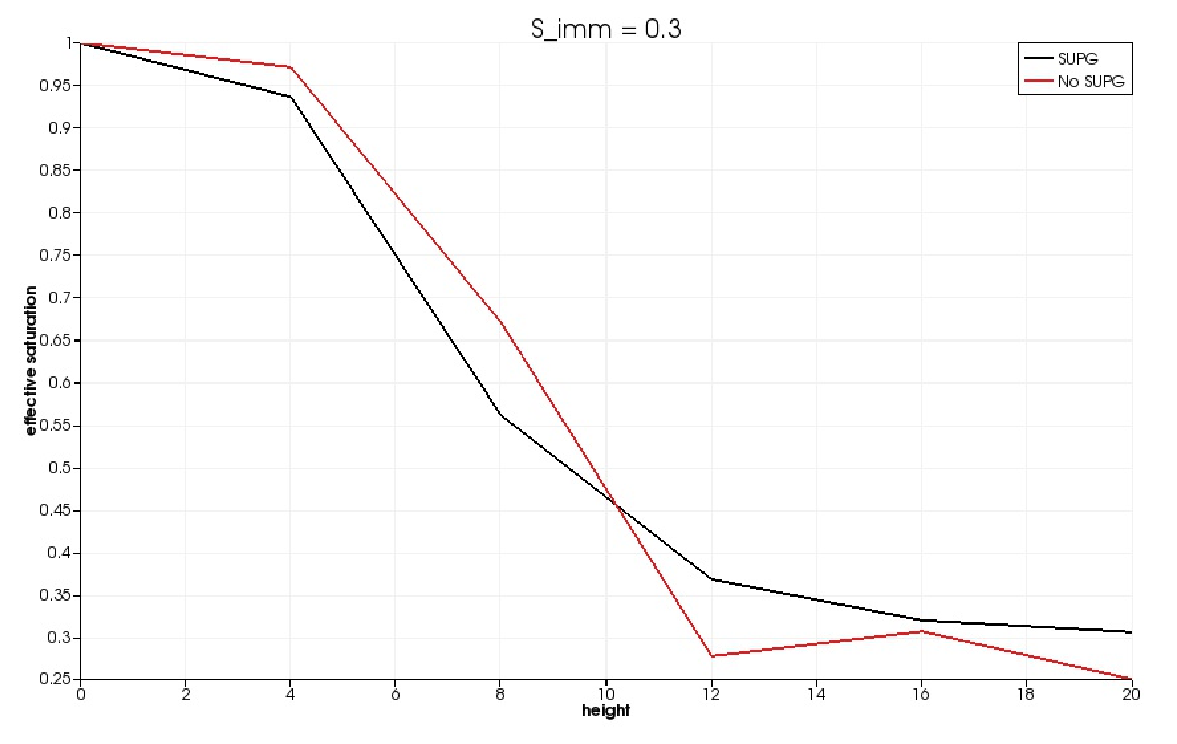
\includegraphics[width=10cm]{gh_seff.eps} \\
$\mbox{}$ \\
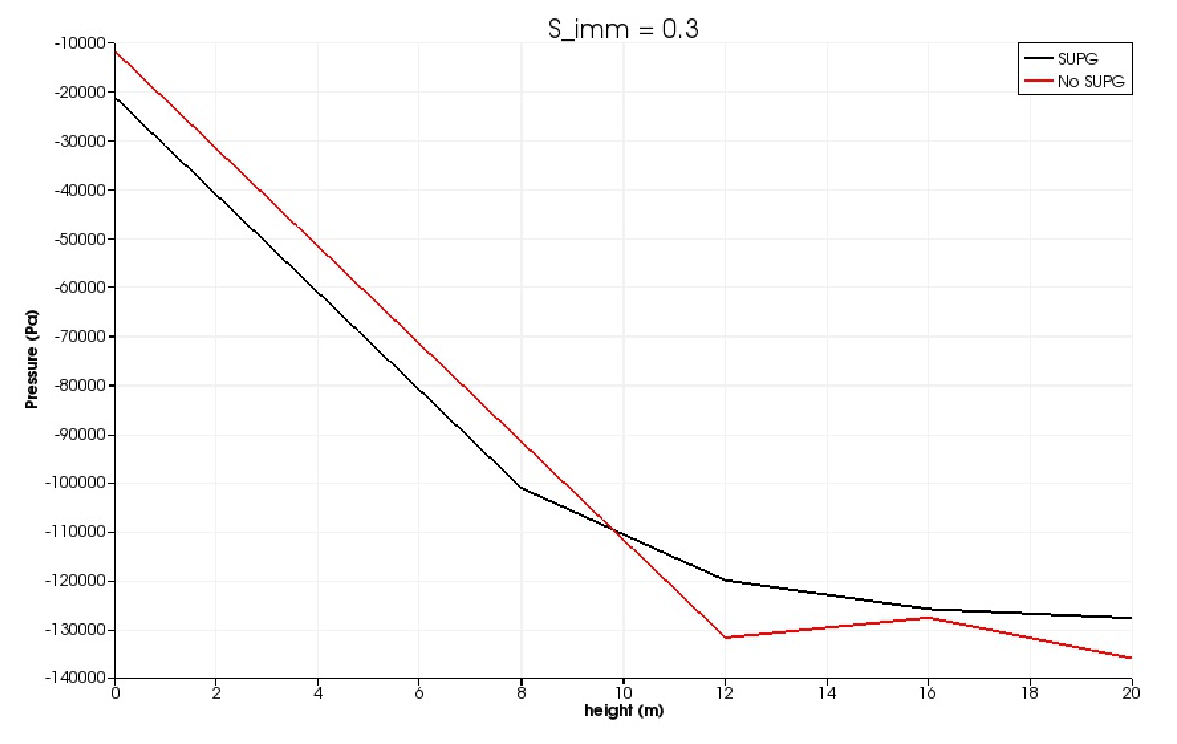
\includegraphics[width=10cm]{gh_p.eps} \\
$\mbox{}$ \\
\begin{tabular}{cc}
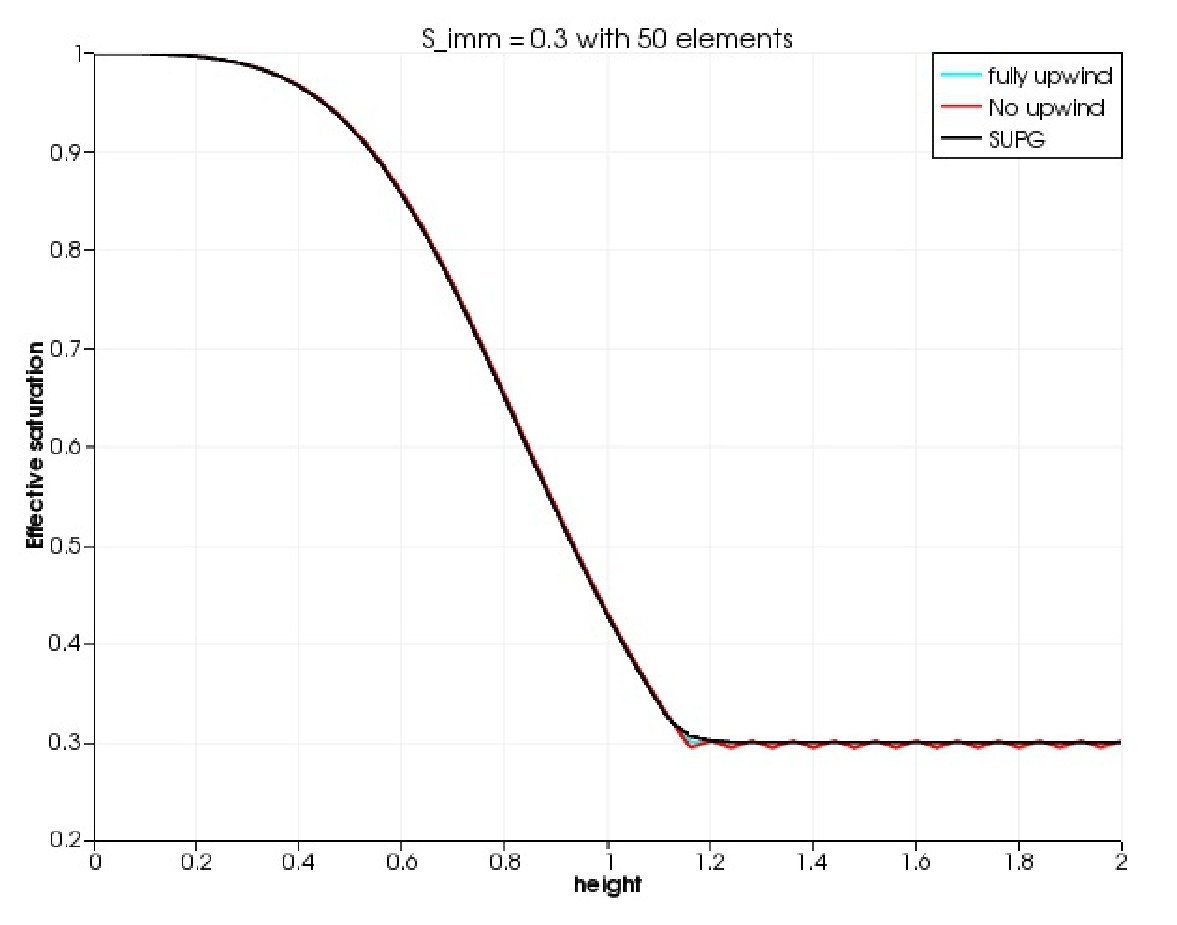
\includegraphics[width=8cm]{gh_seff_50.eps} &
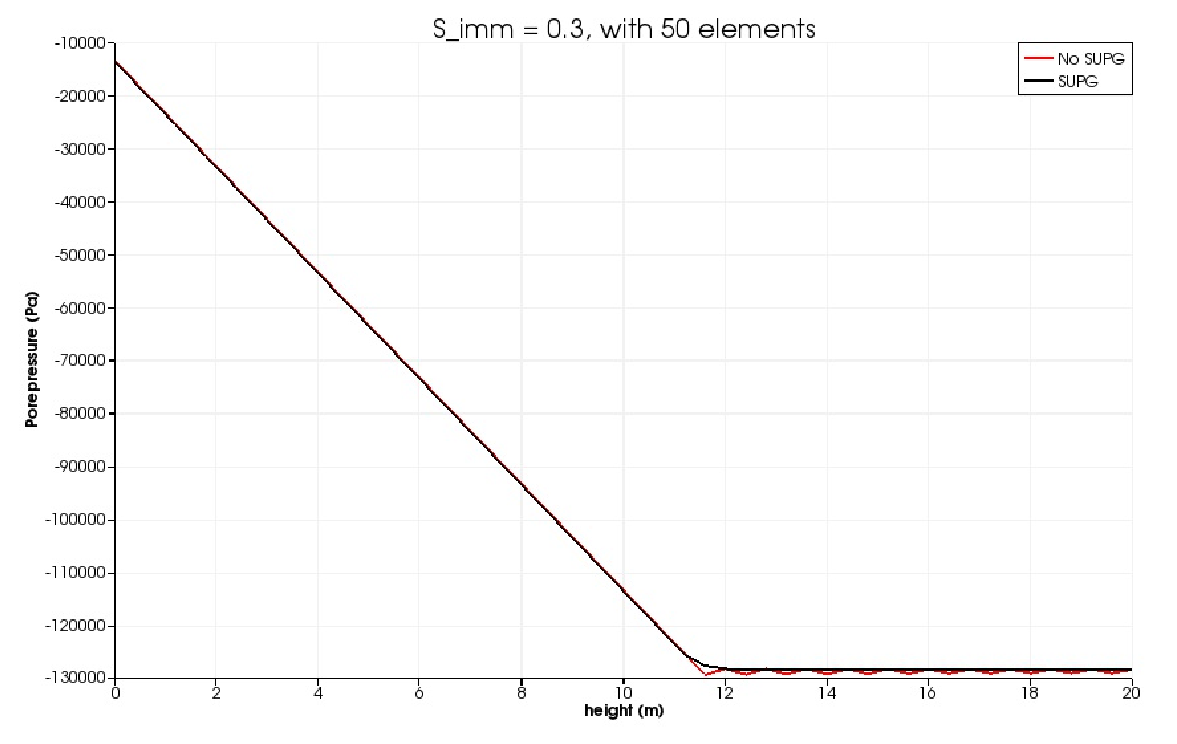
\includegraphics[width=8cm]{gh_p_50.eps} 
\end{tabular}
\caption{Results for $S_{\mathrm{imm}}=0.3$.  Gravity points to the
  left.  Top picture: Effective saturation.  Middle picture: Pore
  pressure.  Bottom pictures: The situation with 50 elements in the
  $x$ direction instead of just 5.  In each picture the red line is
  without SUPG, and oscillatory results can be observed in addition to
  $S_{\mathrm{eff}}< S_{\mathrm{imm}}$.}
\label{gh.fig}
\end{figure}


\chapter{A pressure pulse in the fully saturated situation - NEEDS UPDATE}

Darcy's equation for flow through a fully saturated medium without
gravity and without sources is 
\begin{equation}
\frac{\partial}{\partial t}\phi\rho = \nabla_{i}\left(\frac{\rho
  \kappa_{ij}}{\mu} \nabla_{j}P \right) \ ,
\end{equation}
with notation described in the Theory Manual.  Using $\rho \propto
\exp(P/K)$, where $K$ is the fluid bulk modulus, Darcy's equation
becomes
\begin{equation}
\frac{\partial}{\partial t}\rho = \nabla_{i}\alpha_{ij}\nabla\rho \ ,
\end{equation}
with 
\begin{equation}
\alpha_{ij} = \frac{\kappa_{ij}B}{\mu\phi} \ .
\end{equation}
Here I've assumed the porosity and bulk modulus are constant in space
and time.

Consider the one-dimensional case were the spatial dimension is the
semi-infinite line $x\geq 0$.  Suppose that initially the pressure is
constant, so that
\begin{equation}
\rho(x, t=0) = \rho_{0} \ \ \ \mbox{for }\ \ x\geq 0 \ .
\end{equation}
Then apply a fixed-pressure Dirichlet boundary condition at $x=0$ so
that
\begin{equation}
\rho(x=0, t>0) = \rho_{\infty}
\end{equation}
The solution of the above differential equation is well known to be
\begin{equation}
\rho(x, t) = \rho_{\infty} + (\rho_{0} -
\rho_{\infty})\,\mbox{Erf}\left( \frac{x}{\sqrt{4\alpha t}} \right) \ ,
\label{eqn.exact.pp}
\end{equation}
where Erf is the error function.

This is verified in Wallaby using the following tests on a line of
100 elements.
\begin{enumerate}
\item Steady state analysis with SUPG, in 3D, to demonstrate that the
  steady-state of $\rho = \rho_{\infty}$ is achieved.
\item Transient analysis with SUPG in 3D.
\end{enumerate}
An example verification is shown in Figure~\ref{pressure_pulse.fig}.

\begin{figure}[htb]
\centering
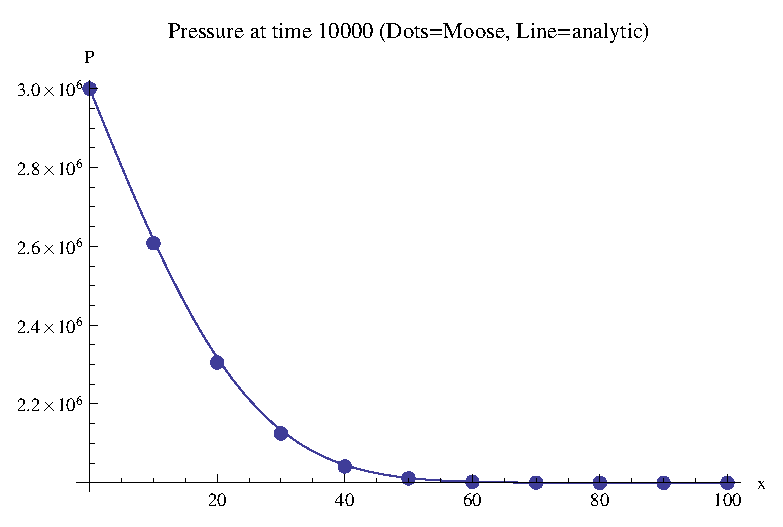
\includegraphics[width=10cm]{pressure_pulse.eps}
\caption{Comparison between the Wallaby result (in dots), and the
  exact analytic expression given by Eqn~(\ref{eqn.exact.pp}).  This
  test had 10 elements in the $x$ direction, with $0\leq x \leq
  100$\,m, and ran for a total of 
  10$^4$ seconds with 10 timesteps.  The parameters were $B=2$\,GPa,
  $\kappa_{xx}=10^{-15}$\,m$^{2}$, $\mu=10^{-3}$\,Pa.s, $\phi=0.1$,
  with initial pressure $P=2$\,MPa, and applied pressure $P=3$\,MPa at
  $x=0$.  For greater spatial resolution and smaller timesteps the
  agreement increases.}
\label{pressure_pulse.fig}
\end{figure}


\chapter{Buckley-Leverett - NEEDS UPDATE}

Wallaby is compared with a simple one dimensional
Buckley-Leverett problem\footnote{SE Buckley and MC Leverett (1942)
  ``Mechanism of fluid displacements in sands''.  Transactions of the
  AIME {\bf 146} 107--116}.  The fluid moves in a region $0\leq x\leq
15$\,m.  A fully-saturated front initially sits at position $x=5$,
while the region $x>5$ is initially unsaturated.  With zero suction
function $P_{c} = 0$, there is no diffusion of the sharp front, and it
progresses towards the right.  This is a difficult problem to simulate
numerically as maintaining the sharp front is hard.  The speed is
independent of the 
relative permeability, since the fluid is flowing from a
fully-saturated region.  This problem is therefore a good test of the upwinding.


In the simulation below, the pressure at the left boundary is kept
fixed at $P_{0}=0.98$\,MPa, while the right boundary is kept fixed at
$P_{15}=-20000$\,Pa.  The medium's permeability is set to $\kappa =
10^{-10}\,\mathrm{m}^{2}$ and its porosity is $\phi = 0.15$.  It is
not possible to use a zero suction function in Wallaby, but using
$\alpha = 10^{-4}$\,Pa$^{-1}$ and $m=0.8$ approximates it.  The fluid
viscosity is $\mu = 10^{-3}$\,Pa.s.

The initial condition is
\begin{equation}
P(t=0) = \left\{
\begin{array}{ll}
P_{0} - (P_{0}-P_{15})x/5 & \ \ \ \mbox{for }\ \ x<5 \\
P_{15} & \ \ \ \mbox{for }\ \ x\geq 5  
\end{array}
\right. \ ,
\end{equation}
which is shown in
Figure~\ref{bl_setup.figa}.  With the suction function defined above
this gives
\begin{equation}
S(t=0) = \left\{
\begin{array}{ll}
1 & \ \ \ \mbox{for }\ \ x\leq 4.9 \\
0.061 & \ \ \ \mbox{for} \ \ x \geq 5
\end{array}
\right.
\end{equation}

\begin{figure}[htb]
\begin{center}
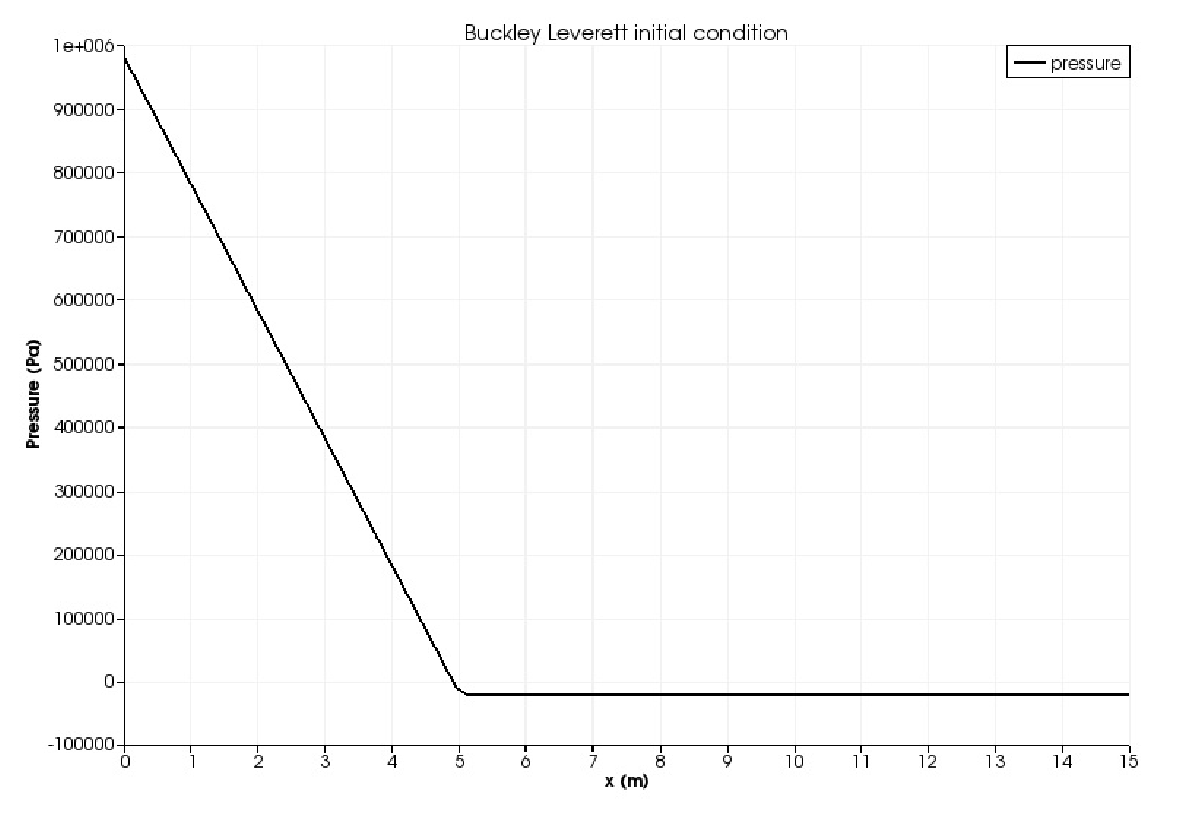
\includegraphics[width=12cm]{bl_initial.eps}
\caption{Initial setup of the Buckley-Leverett problem where
  porepressure is a piecewise linear function.  The region
$x\leq 4.9$ is fully saturated, while the region $x>5$ has saturation
  0.061.  During simulation the value $P(x=0)=0.98\times 10^{6}$\,MPa
  is held fixed.}
\label{bl_setup.figa}
\end{center}
\end{figure}

Good approximations for the pressure $P(x,t)$
and the front position $f(t)$ may be determined from
\begin{eqnarray}
\frac{{\mathrm d} f}{{\mathrm d} t} & = & -\frac{\kappa}{\phi\mu}
\left.\frac{\partial  P}{\partial x}\right|_{x = f} \ , \nonumber \\
P(x,t) & = & \left\{
\begin{array}{ll}
P_{0} - (P_{0}-P_{15})x/f & \mbox{ for } x\leq f  \\
P_{15} & \mbox{ for } x>f 
\end{array}
\right. \ ,
\label{eqn.predicted.bl.posn.eqna}
\end{eqnarray}
which has solution
\begin{equation}
f(t) = \sqrt{f(0)^{2} + \frac{2\kappa}{\phi\mu}(P_{0}-P_{15})t} \ .
\end{equation}
For the parameters listed above, the front will be at position
$f=9.6$\,m at $t=50$\,s.  This solution is only valid for zero
capillary suction.  A nonzero suction function will tend to diffuse
the sharp front away.

With coarse meshes it is impossible to simulate a sharp front, of
course, since the front is spread over at least one element.  It is
therefore quite advantageous to use mesh adaptivity in this test,
since the mesh can be fine around the front where all the interesting
dynamics occurs, and coarse elsewhere.

Figure~\ref{satfront.figa} shows the results from a Wallaby simulation
with an initial mesh of element size 1\,m, and a minimum size of
0.125\,m, with a maximum timestep of 0.3\,s.  (Reducing the minimum
element size or the maximum timestep size keeps the front sharper.)
The front in this simulation is between $x=9.9$\,m and $x=10.35$\,m,
in fair agreement with the predicted value of 9.6\,m.

\begin{figure}[htb]
\begin{center}
\includegraphics[width=10cm]{bl_seff.eps} \\
$\mbox{}$
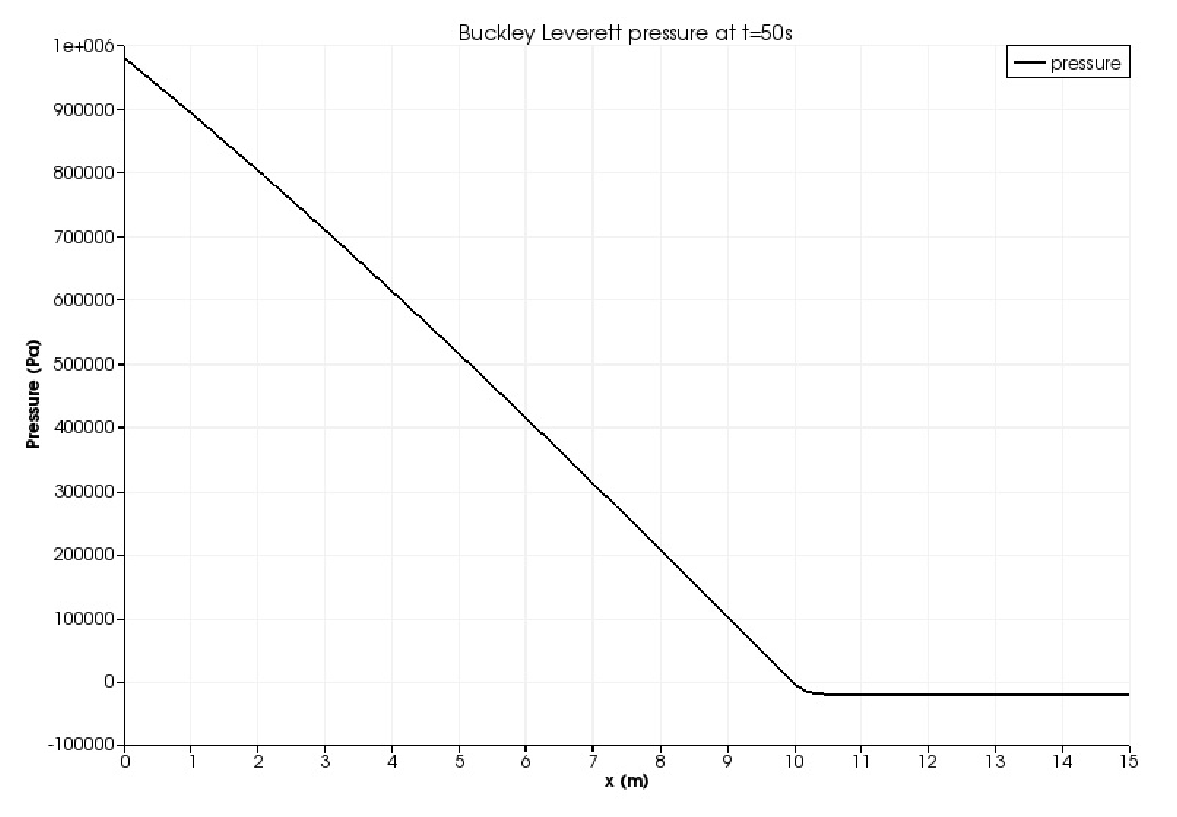
\includegraphics[width=10cm]{bl_p.eps} \\
\caption{The Wallaby solution of the Buckley-Leverett problem at
  $t=50$\,s.  Top: saturation.  Bottom: porepressure.  The front sits
  between $x=9.9$\,m and $x=10.35$\,m.}
\label{satfront.figa}
\end{center}
\end{figure}


\chapter{Unsaturated flow in a bar - NEEDS UPDATE}

This problem is one of cosflow's benchmark problems.  Water inside a
porous ``bar'' of material length 10m, and width and depth 1m is
initialised to porepressure $P_{0}<0$, corresponding to water
saturation $S_{0}<1$.  The porepressure left-hand end (at $x=0$) is
raised and fixed at $P_{1}<0$, corresonding to water saturation
$S_{1}$ with $S_{0}<S_{1}<1$, and the evolution of porepressure at the
right-hand end ($x=10$\,m) is recorded.  Apart from the left-hand end,
the other boundaries of the bar are impermeable.  The setup is shown in
Figure~\ref{uf_setup.fig}.

\begin{figure}[htb]
\begin{center}
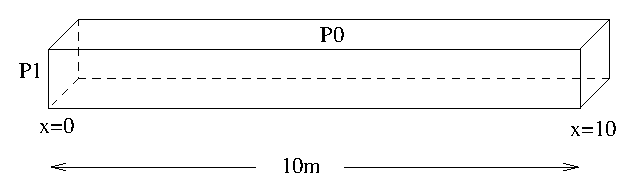
\includegraphics[width=8cm]{uf_setup.eps}
\caption{The unsaturated problem involves a porous
  ``bar'' of material of length 10m with initial porepressure
  $P_{0}$.  The left-hand end is raised to porepressure $P_{1}$ and
  held fixed.  The other parts of the bar's exterior surface are impermeable.}
\label{uf_setup.fig}
\end{center}
\end{figure}

This problem exhibits quite severe mesh dependency, and since the
upwinding in cosflow and Wallaby are different, the results are not
expected to be the same, except in the limit of zero element size.

\noindent The following parameters are used \\
\begin{center}
\begin{tabular}{|ll|}
\hline
Bar porosity & 0.1 \\
Bar permeability & $10^{-12}$\,m$^{2}$ \\
\hline
Gravity & 0 \\
\hline
Water density & 1000\,kg.m$^{-3}$ \\
Water viscosity & 0.001\,Pa.s \\
Water bulk modulus & 2\,GPa \\
Water immobile saturation & 0.0 \\
Water residual saturation & 0.0 \\
Air residual saturation & 0.0 \\
\hline
van Genuchten $\alpha$ & $10^{-4}$\,Pa$^{-1}$ \\
van Genuchten $a$ & 0.35 \\
\hline
Initial porepressure $P_{0}$ & -197347.0503\,Pa \\
Initial saturation $S_{0}$ & 0.2 \\
Applied pressure $P_{1}$ & -9283.000501\,Pa \\
Applied saturation $S_{1}$ & 0.8 \\
\hline
\end{tabular} \\
\end{center}

Figure~\ref{uf.result.fig} shows agreement between Wallaby and
cosflow for a variety of different mesh densities, including an
adaptive mesh example.  The Wallaby results appear to be closer to the
zero-element-size result than cosflow, but for low mesh density
exhibit spurious oscillations as the high saturation region moves into
the low saturation region.  (This oscillation is almost definitely due
to my current inability to lump the mass term.)

\begin{figure}[htb]
\begin{center}
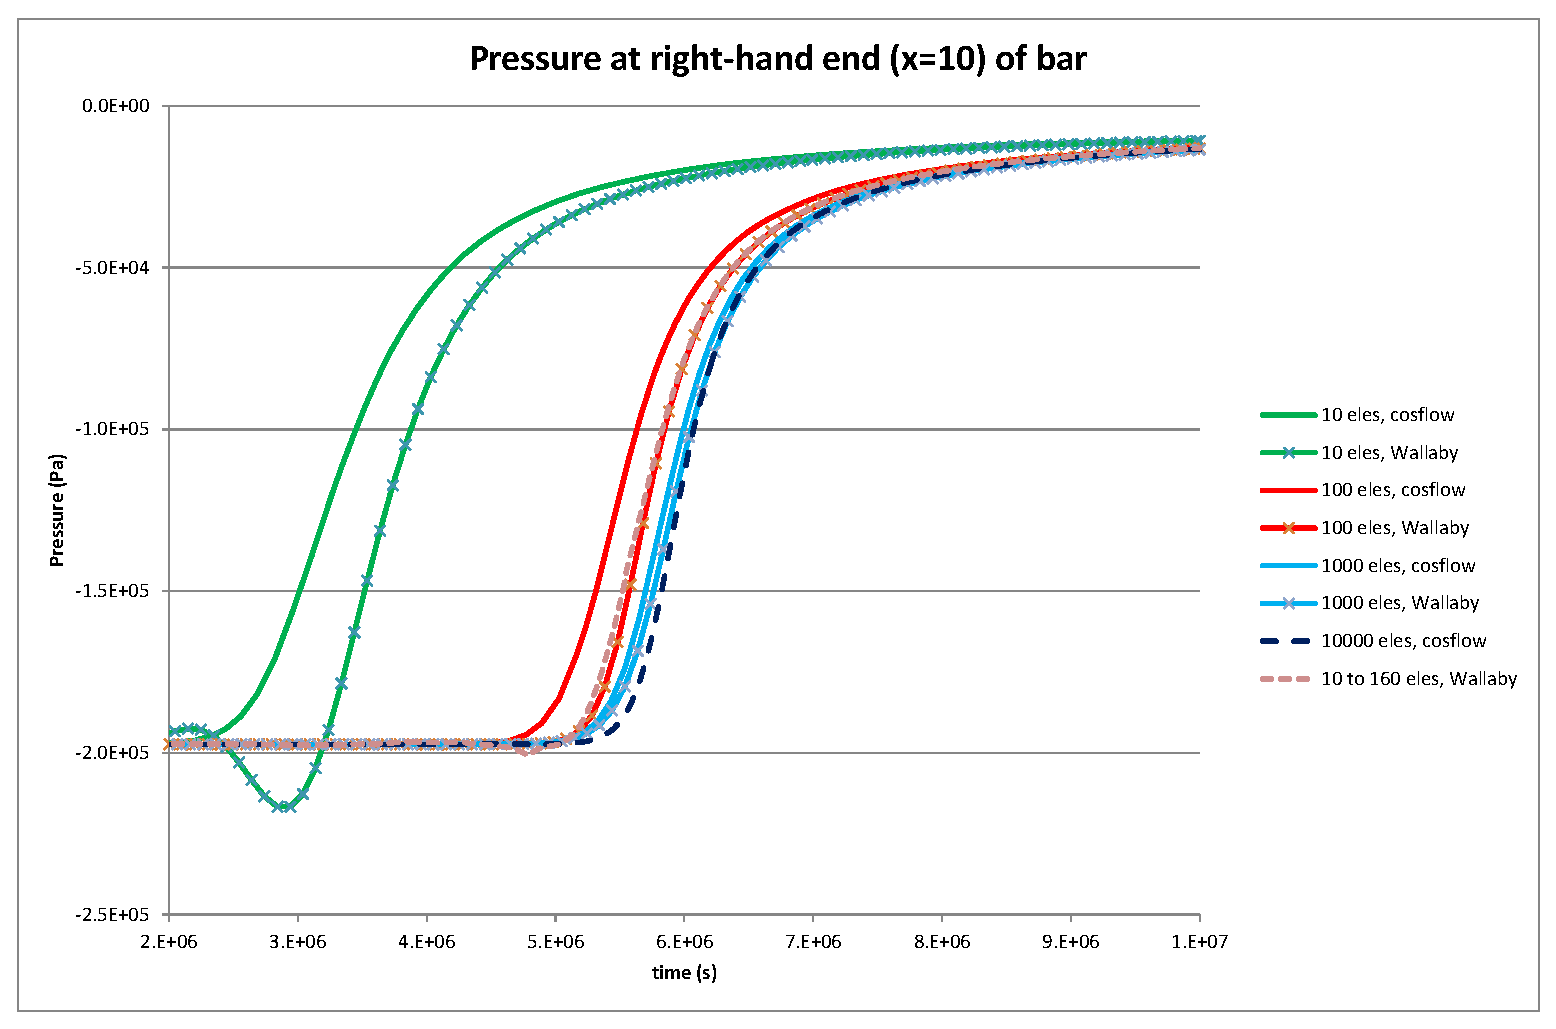
\includegraphics[width=17cm]{uf.eps}
\caption{The porepressure at the right-hand end ($x=10$) of the bar as
  a function of time for various different meshes.}
\label{uf.result.fig}
\end{center}
\end{figure}


\chapter{Infiltration and drainage - NEEDS UPDATE}

Forsyth, Wu and Pruess\footnote{PA Forsyth, YS Wu and K Pruess,
  ``Robust numerical methods for saturated-unsaturated flow with dry
  initial conditions in heterogeneous media'', Advances in Water
  Resources 18 (1995) 25--38} describe a HYDRUS simulation of an
experiment involving infiltration (experiment 1) and subsequent
drainage (experiment 2) in a large caisson.  The simulation is
effectively one dimensional, and is shown in
Figure~\ref{rd_setup.fig}.

\begin{figure}[htb]
\begin{center}
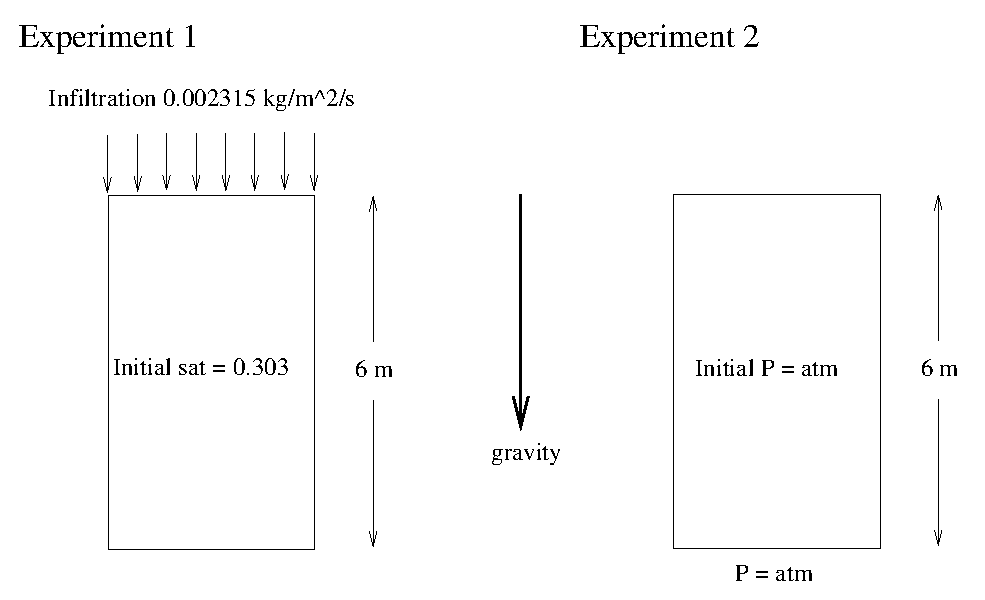
\includegraphics[width=12cm]{rd_setup.eps}
\caption{Two experimental setups from Forsyth, Wu and Pruess.
  Experiment 1 involves infiltration of water into an initially
  unsaturated caisson.  Experiment 2 involves drainage of water from
  an initially saturated caisson.}
\label{rd_setup.fig}
\end{center}
\end{figure}

The properties common to each experiment
are:
\begin{center}
\begin{tabular}{|ll|}
\hline
Caisson & 0.33 \\
Caisson permeability & $2.95\times 10^{-13}$\,m$^{2}$ \\
\hline
Gravity & 10\,m.s$^{-2}$ \\
\hline
Water density & 1000\,kg.m$^{-3}$ \\
Water viscosity & 0.00101\,Pa.s \\
Water bulk modulus & 20\,MPa \\
Water immobile saturation & 0.0 \\
Water residual saturation & 0.0 \\
Air residual saturation & 0.0 \\
Air pressure & 0.0 \\
\hline
van Genuchten $\alpha$ & $1.43\times 10^{-4}$\,Pa$^{-1}$ \\
van Genuchten $a$ & 0.336 \\
van Genuchten\_1 cutoff & 0.99 \\
\hline
\end{tabular} \\
\end{center}
In each experiment 120 finite elements were used along the length of
the Caisson.  The modified van-Genuchten relative permeability curve
was employed in order to improve convergence significantly.  Hydrus
also uses a modified van-Genuchten curve, although I couldn't find any
details on the modification.

In experiment 1, the caisson is initially at saturation 0.303
($P=-72620.4$\,Pa), and water is pumped into the top with a rate
0.002315\,kg.m$^{-2}$.s$^{-1}$.  This causes a front of water to
advance down the caisson.  Figure~\ref{rd.result.fig} shows the
agreement between Wallaby and the published result (this result was
obtained by extracting data by hand from online graphics).

In experiment 2, the caisson is initially fully saturated at $P=0$,
and the bottom is held at $P=0$ to cause water to drain via the action
of gravity.  Figure~\ref{rd.result.fig} shows the agreement between
Wallaby and the published result.


\begin{figure}[htb]
\begin{center}
\includegraphics[width=12cm]{rd01.eps} \\
$\mbox{}$\\
\includegraphics[width=12cm]{rd02.eps}
\caption{Saturation profiles in the caisson.  Top: After 4.16 days of
  infiltration.  Bottom: After drainage from an initially-saturated
  simulation (4 days and 100 days profiles).  Note that the HYDRUS
  results are only approximate as I extrated the data by hand from
  online graphics.}
\label{rd.result.fig}
\end{center}
\end{figure}


\chapter{Newton cooling from a bar - NEEDS UPDATE}

Darcy's equation for flow through a fully saturated medium without
gravity and without sources is 
\begin{equation}
\frac{\partial}{\partial t}\phi\rho = \nabla_{i}\left(\frac{\rho
  \kappa_{ij}}{\mu} \nabla_{j}P \right) \ ,
\end{equation}
with notation described in the Theory Manual.  Using $\rho \propto
\exp(P/K)$, where $K$ is the fluid bulk modulus, Darcy's equation
becomes
\begin{equation}
\frac{\partial}{\partial t}\rho = \nabla_{i}\alpha_{ij}\nabla\rho \ ,
\end{equation}
with 
\begin{equation}
\alpha_{ij} = \frac{\kappa_{ij}B}{\mu\phi} \ .
\end{equation}
Here I've assumed the porosity and bulk modulus are constant in space
and time.

Consider the one-dimensional case where a bar sits between $x=0$ and
$x=L$ with initial pressure distribution so $\rho(x,t=0) = \rho_{0}(x)$.
Maintain the end $x=0$ at constant pressure, so that $\rho(x=0, t) =
\rho_{0}(0)$.  At the end $x=L$, prescribe a sink flux
\begin{equation}
\left.\frac{\partial\rho}{\partial x}\right|_{x=L} = -C\left(\rho -
\rho_{e}\right)_{x=L} \ ,
\end{equation}
where $\rho_{e}$ is a fixed quantity (``e'' stands for ``external''),
and $C$ is a constant conductance.  This corresponds to the flux
\begin{equation}
\left.\frac{\partial P}{\partial x}\right|_{x=L} = -CB\left(1 -
e^{(P_{e}-P)/B}\right)_{x=L} \ ,
\end{equation}
which can easily be coded into a Wallaby input file: the flux is
$\rho\kappa\nabla P/\mu = -CB\kappa(e^{P/B} - e^{P_{e}/B})/\mu$.

The solution of this problem is well known and is
\begin{equation}
\rho(x, t) = \rho_{0}(0) - \frac{\rho_{0}(0) - \rho_{e}}{1 + LC}Cx +
\sum_{n=1}^{\infty} a_{n}\sin \frac{k_{n}x}{L}e^{-k_{n}^{2}\alpha
  t/L^{2}} \ ,
\end{equation}
where $k_{n}$ is the $n^{\mathrm{th}}$ positive root of the equation
$LC\tan k + k=0$  ($k_{n}$ is a little bigger than
$(2n-1)\pi/2$), and $a_{n}$ is determined from
\begin{equation}
a_{n}\int_{0}^{L}\sin^{2}\frac{k_{n}x}{L}\,\mathrm{d}x =
\int_{0}^{L}\left(\rho_{0}(x) - \rho_{0}(0) + \frac{\rho_{0}(0) -
  \rho_{e}}{1 + LC}Cx\right)\sin \frac{k_{n}x}{L}\,\mathrm{d}x \ ,
\end{equation}
which may be solved numerically.

\noindent The problem is solved in Wallaby using the following parameters:
\begin{center}
\begin{tabular}{|ll|}
\hline
Bar length & 100\,m \\
Bar porosity & 0.1 \\
Bar permeability & $10^{-15}$\,m$^{2}$ \\
\hline
Gravity & 0 \\
\hline
Water density & 1000\,kg.m$^{-3}$ \\
Water viscosity & 0.001\,Pa.s \\
Water bulk modulus & 1\,MPa \\
\hline
Initial porepressure $P_{0}$ & 2\,MPa \\
Environmental pressure $P_{e}$ & 0 \\
\hline
Conductance $C$ & 0.05389\,m$^{-1}$ \\
\hline
\end{tabular} \\
\end{center}
This conductance is chosen so at steadystate $\rho(x=L)=2000$\,kg.m$^{-3}$.

The problem is solved using 1000 elements along the $x$
direction ($L=100$\,m), and using 100 time-steps of size $10^6$\,s.
Using fewer elements or fewer timesteps means the agreement with the
theory is marginally poorer.  The problem is also solved using the
steadystate solver.  In this case the initial condition is
$P=2-x/L$\,MPa, since the uniform $P=2$\,MPa does not converge.  The
results are shown in Figure~\ref{nc.fig}.

\begin{figure}[htb]
\begin{center}
\includegraphics[width=17cm]{nc.eps}
\caption{The porepressure in the bar at $t=10^{8}$\,s, and at
  steadystate.  Wallaby agrees well with theory.}
\label{nc.fig}
\end{center}
\end{figure}







\chapter{Future tests}

See ''Benchmarking of Richards Model'' Yanlian Du, Wenqing Wang and
Olaf Kolditz for a summary of the usual suspects.

See Forsyth, Wu and Pruess for more tests.








\end{document}

